\subsection{analoges Theremin}\label{subsec:Theremin_analog}
Das klassische Theremin besitzt zwei Antennen. Der Spieler kann über die senkrecht angebrachte Antenne  die  Tonhöhe beeinflussen. Mit der waagrechten Antenne beeinflusst der Spieler die Lautstärke. Eine typische Eigenschaft des Theremin ist, dass der Ton des Theremin in einem weitem Frequenzbereich kontinuierlich veränderbar ist. Das Theremin ist daher nicht auf die Tonleiter beschränkt.

Das Theremin erzeugt Töne durch das verstimmen des an der Antenne angebrachten Oszillators.
 Die Hand des Spielers, der durch seine eigene Masse als Erdung fungiert, verändert über die jeweilige Antenne den LC-Schwingkreis des Tonhöhen und Lautstärkeoszillators. Dabei wird der kapazitive Anteil des Schwingkreis beeinflusst, was eine Änderung der Schwingfrequenz zur Folge hat. 
 Die Frequenz dieser Oszillatoren ist jedoch weit über dem hörbaren Bereich (zwischen \SI{100}{kHz} bis \SI{1}{MHz}). Mit Hilfe eines Mischers und einem Referenzoszillator wird die Frequenzdifferenz hörbar gemacht und danach verstärkt\cite{Franzis}. Die Abbildung \ref{img:Blockschaltbild_analog} gibt einen Überblick über die Schaltungskomponenten eines Theremins. Die einzelnen Schaltungsteile sind im folgenden Teil genauer erklärt.

\begin{figure}[h]
	\centering
	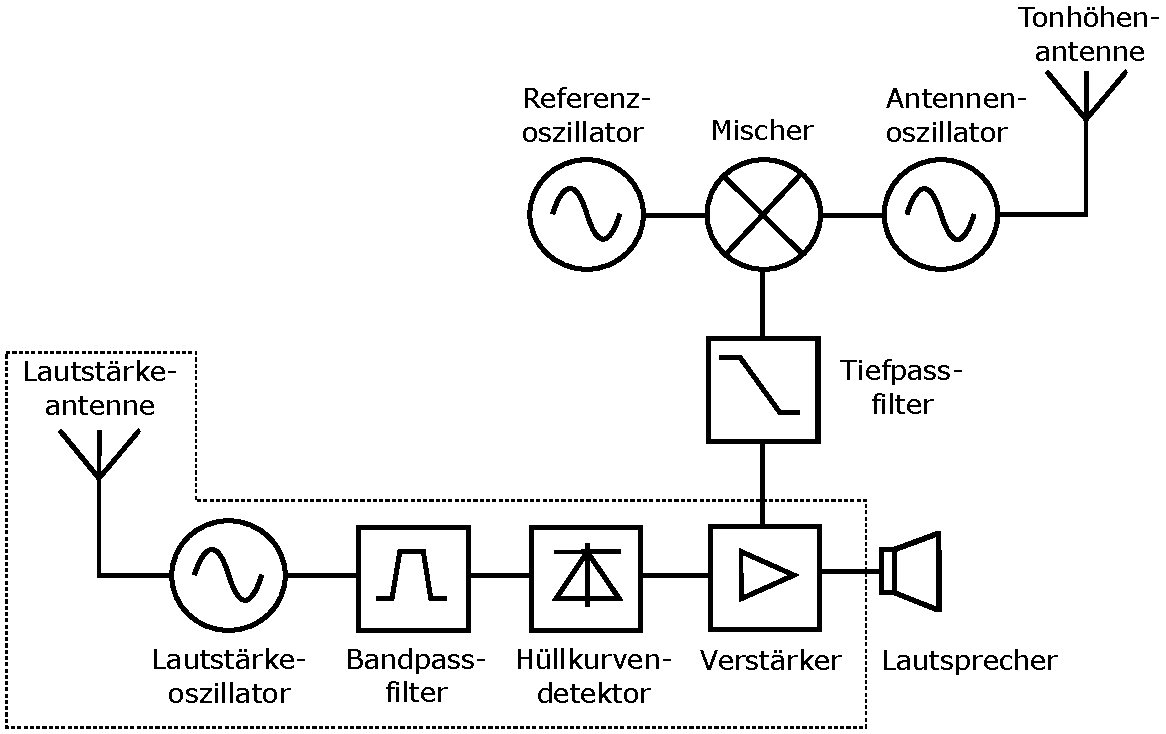
\includegraphics[width=\textwidth]{Blockschaltbild_analog.pdf}
	\caption{Blockschaltbild eines analogen Theremins}
	\label{img:Blockschaltbild_analog}
\end{figure}

\paragraph{Tonhöhenoszillator und Tonhöhenantenne}\mbox{}
\\Die Tonhöhenantenne ist ein Metallrohr welches mit dem Antennenoszillator verbunden ist.
Durch die Hand des Spielers wird über die Tonhöhenantenne die Frequenz des Antennenoszillators verändert. Die Kapazitätsänderung welche über die Antenne erreicht werden kann ist sehr gering. Diese liegt im Picofarad Bereich \cite{physik_theremin}. Um eine genug grosse Frequenzänderung zu erzeugen muss demnach die Grundfrequenz des Antennenoszillators weit über dem hörbaren Frequenzbereich gewählt werden. 

\paragraph{Lautstärkeoszillator und Lautstärkeantenne}\mbox{}\\ 
Die Lautstärkeantenne ist wie die Tonhöhenantenne ein Metallrohr, welches mit dem Tonhöhenoszillator verbunden ist. Die durch den Spieler beeinflusste Frequenzänderung wandelt ein Hüllkurvendetektor in eine Spannungsänderung um. Diese Spannungsänderung dient dem Verstärker als Steuergrösse um das Audio Signal zu verstärken. \cite{Franzis}. 

\paragraph{Mischer und Referenzoszillator}\mbox{}\\ 
\\Die erzeugte Frequenz der Tonhöhenantenne ist weit über dem vom Menschen hörbaren Bereich. Deswegen wird das Antennen Signal mit einem Referenzoszillator mit fester Frequenz gemischt. Dies bewirkt eine Frequenzdifferenz im hörbaren Bereich.
Um diese Differenz zu erhalten multipliziert der Mischer die zwei Signale des Referenzoszillator $A_1\sin(\omega_1)$  und des Antennenoszillator $A_2\sin(\omega_2)$ wie folgt:

\begin{equation}
V_{out} = A_{1}A_{2} \sin(\omega_{1}t)   \sin(\omega_{2}t) 
\label{equ:mischer}
\end{equation}

$V_{out}$ kann durch Additionstheoreme umgeformt werden. Dabei erhält man folgenden Ausdruck:

\begin{equation}
V_{out} = A/2[\cos((\omega_{1}-\omega_{2})t)  - \cos((\omega_{1}+\omega_{2})t) ]
\label{equ:mischer_trigo}
\end{equation}

Das Ausgangssignal $V_{out}$ hat zwei Frequenzkomponenten. Zum einen die Differenz der beiden Frequenzen zum anderen die Summe der Frequenzen. Dabei ist bei dem Theremin nur die Differenz der Frequenzen von Interesse \cite{physik_theremin}.

Das Theremin muss vor jedem Gebrauch kalibriert werden. Es könnte beispielsweise sein, dass die Differenz der Frequenz ausserhalb des hörbaren Bereiches ist. Dazu wird beim klassischen Theremin mit Hilfe eines Trimmkondensators am Referenzoszillator die Differenzfrequenz auf \SI{0}{Hz} gestellt.

\paragraph{Tiefpassfilter}\mbox{}\\ 
\\Mit Hilfe eines Tiefpassfilters wird das Signal mit der Summe der Oszillator Frequenzen vollständig abgeschwächt. Übrig bleibt die Differenz der Oszillator Frequenzen. Dieser ist der Anteil des Mischprozesses, welcher von Intresse ist, da er im hörbaren Bereich ist.
\begin{equation}
V_{out} = A/2cos((\omega_{1}-\omega_{2})t) 
\label{equ:mischer_trigo}
\end{equation}

\paragraph{Verstärker und  Lautsprecher}\mbox{}\\ 
\\Die hörbare Differenz wird verstärkt und über einen Lautsprecher ausgegeben.
